%!TEX program = xelatex

\documentclass[a4paper,14pt]{extarticle}
\author{Хутиев Рустэм Русланович \\ Куликовских Денис}
\title{Поиск оптимального равновесия на рынке такси}

\date{\today}

\usepackage{comment} % Многострочный комментарий

\usepackage[english,russian]{babel} %% загружает пакет многоязыковой вёрстки
\usepackage{fontspec} %% подготавливает загрузку шрифтов Open Type, True Type и др.

\usepackage{indentfirst}
\usepackage{tcolorbox}

\defaultfontfeatures{Ligatures={TeX},Renderer=Basic} %% свойства шрифтов по умолчанию
\setmainfont[Ligatures={TeX,Historic}]{Times New Roman} %% задаёт основной шрифт документа
\setmonofont{Courier New}
\frenchspacing

\renewcommand{\epsilon}{\ensuremath{\varepsilon}}
\renewcommand{\phi}{\ensuremath{\varphi}}
\renewcommand{\kappa}{\ensuremath{\varkappa}}
\renewcommand{\le}{\ensuremath{\leqslant}}
\renewcommand{\leq}{\ensuremath{\leqslant}}
\renewcommand{\ge}{\ensuremath{\geqslant}}
\renewcommand{\geq}{\ensuremath{\geqslant}}
\renewcommand{\emptyset}{\varnothing}

%%% Дополнительная работа с математикой
\usepackage{amsmath,amsfonts,amssymb,amsthm,mathtools} % AMS
\usepackage{float}
\usepackage{icomma} % "Умная" запятая: $0,2$ --- число, $0, 2$ --- перечисление
\usepackage{mathtext} % Русские буквы в матрежиме
\usepackage{dsfont} % Математически символы
\usepackage{pgfplots}
\usepackage{algorithm}
\usepackage{algpseudocode}

\pgfplotsset{compat=1.18}
%% Номера формул
%\mathtoolsset{showonlyrefs=true} % Показывать номера только у тех формул, на которые есть \eqref{} в тексте.
%\usepackage{leqno} % Нумерация формул слева

%% Свои команды
\DeclareMathOperator{\sgn}{\mathop{sgn}}

%% Перенос знаков в формулах (по Львовскому)
\newcommand*{\hm}[1]{#1\nobreak\discretionary{}
{\hbox{$\mathsurround=0pt #1$}}{}}

%%% Работа с картинками
\usepackage{graphicx}  % Для вставки рисунков
\graphicspath{{images/}{images2/}}  % папки с картинками
\setlength\fboxsep{3pt} % Отступ рамки \fbox{} от рисунка
\setlength\fboxrule{1pt} % Толщина линий рамки \fbox{}
\usepackage{wrapfig} % Обтекание рисунков текстом

%%% Работа с таблицами
\usepackage{array,tabularx,tabulary,booktabs} % Дополнительная работа с таблицами
\usepackage{longtable}  % Длинные таблицы
\usepackage{multirow} % Слияние строк в таблице

%%% Теоремы
\theoremstyle{plain} % Это стиль по умолчанию, его можно не переопределять.
\newtheorem{theorem}{Теорема}[section]
\newtheorem{proposition}[theorem]{Утверждение}
 
\theoremstyle{definition} % "Определение"
\newtheorem{corollary}{Следствие}[theorem]
\newtheorem{problem}{Задача}[section]
 
\theoremstyle{remark} % "Примечание"
\newtheorem*{nonum}{Решение}

%%% Программирование
\usepackage{etoolbox} % логические операторы

%%% Страница
\usepackage{indentfirst} % Красная строка
\usepackage{extsizes} % Возможность сделать 14-й шрифт
\usepackage{geometry} % Простой способ задавать поля
\geometry{top=2cm, bottom=2cm, left=2.5cm, right=2.5cm}

\begin{comment}
\usepackage{fancyhdr} % Колонтитулы
\pagestyle{fancy}
%\renewcommand{\headrulewidth}{0pt}  % Толщина линейки, отчеркивающей верхний колонтитул
\lfoot{Нижний левый}
\rfoot{Нижний правый}
\rhead{Верхний правый}
\chead{Верхний в центре}
\lhead{Верхний левый}
\cfoot{Нижний в центре} % По умолчанию здесь номер страницы
\end{comment}

\usepackage{setspace} % Интерлиньяж
\onehalfspacing % Интерлиньяж 1.5
%\doublespacing % Интерлиньяж 2
%\singlespacing % Интерлиньяж 1

\usepackage{lastpage} % Узнать, сколько всего страниц в документе.

\usepackage{caption} % Капция

\usepackage{soul} % Модификаторы начертания

\usepackage{hyperref}
\usepackage{xcolor}
\hypersetup{				% Гиперссылки
	unicode=true,           % русские буквы в раздела PDF
	pdftitle={Заголовок},   % Заголовок
	pdfauthor={Автор},      % Автор
	pdfsubject={Тема},      % Тема
	pdfcreator={Создатель}, % Создатель
	pdfproducer={Производитель}, % Производитель
	pdfkeywords={keyword1} {key2} {key3}, % Ключевые слова
	colorlinks=true,       	% false: ссылки в рамках; true: цветные ссылки
	linkcolor=black,          % внутренние ссылки
	citecolor=black,        % на библиографию
	filecolor=magenta,      % на файлы
	urlcolor=black           % на URL
}

\usepackage{csquotes} % Еще инструменты для ссылок

%%% Библиография

\usepackage{multicol} % Несколько колонок

\usepackage{tikz} % Работа с графикой
\usepackage{pgfplots}
\usepackage{pgfplotstable}

%%% Программный код
\usepackage{listings}
\usepackage{minted}

\definecolor{codegreen}{rgb}{0,0.6,0}
\definecolor{codegray}{rgb}{0.5,0.5,0.5}
\definecolor{codepurple}{rgb}{0.58,0,0.82}
\definecolor{backcolour}{rgb}{0.95,0.95,0.92}
\definecolor{codeorange}{rgb}{1,0.25,0}

\lstdefinestyle{mystyle}{
inputencoding=utf8x,
backgroundcolor=\color{backcolour},   
commentstyle=\color{codegreen},
keywordstyle=\color{codeorange},
numberstyle=\tiny\color{codegray},
stringstyle=\color{codepurple},
basicstyle=\ttfamily\footnotesize,
breakatwhitespace=false,         
breaklines=true,                 
captionpos=t,                    
keepspaces=true,                 
numbers=left,                    
numbersep=5pt,                  
showspaces=false,                
showstringspaces=false,
showtabs=false,                  
tabsize=2,
}

\lstset{style=mystyle}

\DeclareCaptionFormat{listing}{#1#2\\#3}
\captionsetup[lstlisting]{justification=centering, format=listing, labelsep=period}
\usepackage{csvsimple}
\usepackage[round]{natbib} 
\setlength{\bibsep}{0.0pt}
\setlength\extrarowheight{2pt} % Дополнительная высота для таблиц

% Темный вариант PDF 
%\pagecolor[rgb]{0,0,0} %black

%\color[rgb]{0.5,0.5,0.5} %grey % Пакеты и параметры документа

\begin{document} % Конец преамбулы, начало документа
\pagenumbering{gobble} % Отключает нумерацию страниц
%!TEX root = main.tex

% НАЧАЛО ТИТУЛЬНОГО ЛИСТА
\begin{center}
    
    \textbf{Федеральное государственное автономное образовательное учреждение высшего образования}

    \textbf{Национальный исследовательский университет \\ <<Высшая школа экономики>>}

    \textbf{Факультет компьютерных наук}
\end{center}

\begin{center}
    \underline{Хутиев Рустэм Русланович}
\end{center}

\begin{center}
    \vspace{5ex}
    \textbf{МАГИСТЕРСКАЯ ДИССЕРТАЦИЯ}
    \vspace{3ex}
    
    \textbf{\underline{Исследование больших языковых моделей для задач рекомендательных систем}}

    \textbf{\underline{Exploring Large Language Models for Recommender Systems}}

    \vspace{3ex}
    по направлению подготовки  \underline{01.04.02 Прикладная математика и информатика}

    образовательная программа \underline{«Финансовые технологии и анализ данных»}
    
    \vspace{10ex}
\end{center}

\begin{flushright} % выравнивание по правому краю

    \begin{flushright} % выровнять её содержимое по левому краю
        Научный руководитель\\
        Доцент ФКН НИУ ВШЭ\\
        А. А. Масютин\\
    \end{flushright}

    \underline{\hspace{5cm}}

    \begin{flushright} % выровнять её содержимое по левому краю
        Соруководитель \\
        Ведущий исследователь-разработчик \\
        О. А. Лашинин
    \end{flushright}

    \underline{\hspace{5cm}}

    \begin{flushright} % выровнять её содержимое по левому краю
        Студент \\
        Хутиев Р. Р
    \end{flushright}
    \underline{\hspace{5cm}}

    
\end{flushright}
\vfill
\begin{center} \small Москва 2025 \end{center}
\thispagestyle{empty}
\pagebreak
 
\tableofcontents 
\newcommand{\anonsection}[1]{\section*{#1}\addcontentsline{toc}{section}{#1}}
\newpage

\section*{Аннотация}

Выпускная квалификационная работа посвящена разработке и оценке эффективности применения больших языковых моделей для решения задачи персонализированных рекомендаций контента. Целью исследования является создание интеллектуальной рекомендательной системы, способной решать проблему замкнутости традиционных подходов и обеспечивать пользователям возможность исследования новых областей интересов.

В рамках работы была разработана двухуровневая архитектура на основе семантической кластеризации контента и адаптации большой языковой модели для генерации персонализированных переходов между кластерами интересов.

Методологическую основу составила гибридная архитектура, объединяющая создание семантических эмбеддингов контента с помощью модели SentenceTransformer, иерархическую кластеризацию на основе алгоритма balanced-split и параметрически-эффективное дообучение языковой модели Llama-3.1-8B с использованием LoRA-архитектуры.

Эмпирическая база включает открытый датасет MTS Kion Dataset, содержащий данные о 5.5 миллионах взаимодействий 962 тысяч пользователей с 15.7 тысячами фильмов.

Полученные результаты демонстрируют высокую эффективность предложенного подхода: дообученная модель достигла значения Article Match Rate на уровне 99.6\%, при этом применение LoRA позволило сократить количество обучаемых параметров до 2.05\% от общего объема модели. Результаты подтверждают способность больших языковых моделей генерировать семантически корректные рекомендации, успешно решая проблему замкнутости рекомендательных систем.

\textbf{Ключевые слова}

Большие языковые модели, рекомендательные системы, иерархическая кластеризация, LoRA, персонализация, семантические эмбеддинги, замкнутость рекомендательных систем 

\newpage
\section*{Abstract}

This thesis is devoted to the development and evaluation of the effectiveness of applying large language models to solve the problem of personalized content recommendations. The research aims to create an intelligent recommendation system capable of addressing the filter bubble problem of traditional approaches and providing users with the opportunity to explore new areas of interest.

A two-level architecture was developed based on semantic content clustering and adaptation of a large language model for generating personalized transitions between interest clusters.

The methodological foundation consisted of a hybrid architecture combining semantic content embeddings creation using the SentenceTransformer model, hierarchical clustering based on the balanced-split algorithm, and parameter-efficient fine-tuning of the Llama-3.1-8B language model using LoRA architecture.

The empirical base includes the open MTS Kion Dataset containing data on 5.5 million interactions of 962 thousand users with 15.7 thousand movies.

The obtained results demonstrate high effectiveness of the proposed approach: the fine-tuned model achieved an Article Match Rate of 99.6\%, while the application of LoRA reduced the number of trainable parameters to 2.05\% of the total model volume. The results confirm the ability of large language models to generate semantically correct recommendations, successfully solving the filter bubble problem of recommendation systems.

\textbf{Keywords}

Large language models, recommendation systems, hierarchical clustering, LoRA, personalization, semantic embeddings, filter bubble problem

\newpage

\pagenumbering{arabic} % Включает нумерацию страниц с 1
\section*{Введение}
\addcontentsline{toc}{section}{Введение}


Рекомендательные системы (РС) стали неотъемлемой частью современных онлайн-платформ, помогая пользователям ориентироваться в огромных объемах информации и находить релевантный контент, продукты или услуги. Традиционные подходы к построению РС, такие как коллаборативная фильтрация и контент-ориентированные методы, достигли значительных успехов, однако они часто сталкиваются с проблемами разреженности данных, холодного старта и ограниченной способностью к пониманию семантических нюансов пользовательских предпочтений и описаний элементов.

В последнее время наблюдается значительный рост интереса к большим языковым моделям (Large Language Models, LLM), которые демонстрируют уникальные способности в понимании, генерации и обработке естественного языка. Это привело к открытию новых горизонтов для различных областей искусственного интеллекта, включая рекомендательные системы. Активно изучается возможность применения LLM для решения классических проблем РС и создания более продвинутых, персонализированных и интерактивных рекомендательных сервисов. Современные исследования выделяют два основных направления применения LLM в рекомендательных системах: дискриминативные модели (DLLM4Rec), ориентированные на классификацию и ранжирование, и генеративные модели (GLLM4Rec), способные создавать персонализированные рекомендации и объяснения в естественном языке \citep{wu2024surveylargelanguagemodels}. Кроме того, появляется интерес к агентным системам, где LLM выступают в роли интеллектуальных агентов, способных к диалоговому взаимодействию и стратегическому планированию рекомендаций \citep{peng2025surveyllmpoweredagentsrecommender}.

Однако, несмотря на значительный потенциал, интеграция LLM в рекомендательные системы сопряжена с рядом вызовов. К ним относятся высокая чувствительность к формулировке запросов, возможность генерации некорректных или несуществующих рекомендаций, а также значительные вычислительные затраты при внедрении в реальные приложения. Тем не менее, активные исследования в этой области продолжаются, предлагая новые архитектурные решения и методы адаптации больших языковых моделей для улучшения качества рекомендаций и повышения доверия пользователей \citep{vats2024exploringimpactlargelanguage}.


\underline{Цель работы:} разработка и оценка эффективности внедрения больших языковых моделей в области рекомендательных систем.

\underline{Задачи работы:}
\begin{itemize}
    \item Провести систематический обзор литературы по применению больших языковых моделей в рекомендательных системах
    \item Разработать методологию создания семантических представлений контента на основе текстовых эмбеддингов и иерархической кластеризации
    \item Реализовать двухуровневую архитектуру рекомендательной системы, использующую LLM для генерации переходов между кластерами интересов
    \item Адаптировать большую языковую модель с использованием LoRA-архитектуры для задачи предсказания пользовательских предпочтений
    \item Провести экспериментальную оценку эффективности предложенного подхода на датасете MTS Kion
    \item Проанализировать способность модели решать проблему замкнутости рекомендательных систем
\end{itemize}

\underline{Методы исследования:}
\begin{itemize}
    \item Анализ литературы и систематизация подходов к применению LLM в рекомендательных системах
    \item Предобработка данных и создание текстовых описаний контента с генерацией ключевых слов через LLM
    \item Создание семантических эмбеддингов с помощью модели SentenceTransformer (Jina-v3) и иерархическая кластеризация контента
    \item Извлечение характеризующих ключевых слов кластеров с использованием TF-IDF анализа
    \item Параметрически-эффективное дообучение языковой модели Llama-3.1-8B с применением LoRA-архитектуры
    \item Разработка специализированных метрик оценки: recall\_exact\_completion, avg\_jaccard\_to\_true, article\_match\_rate
    \item Количественный и качественный анализ результатов генерации рекомендаций
\end{itemize}

\underline{Объект исследования:} набор реальных данных из приложения МТС Kion по взаимодействиям пользователей с контентом за период 6 месяцев в 2021 году, включающий в себя факты просмотра контента пользователями, описания различных аттрибутов контента, а также описательные метрики пользователя\footnote{MTS Kion Implicit Contextualised Sequential Dataset for Movie Recommendation // URL: \url{https://github.com/irsafilo/KION_DATASET?tab=readme-ov-file}}.

\underline{Актуальность работы:} заключается в анализе и применении передовых подходов в задаче использования LLM для рекомендации контента, что позволяет повысить качество персонализации и решить классические проблемы рекомендательных систем.  % Введение
\newpage

\section*{Обзор литературы}
\addcontentsline{toc}{section}{Обзор литературы}
\subsection*{LLM в контентно-ориентированных и коллаборативных рекомендациях}
\addcontentsline{toc}{subsection}{LLM в контентно-ориентированных и коллаборативных рекомендациях}

Традиционные рекомендательные системы основываются на двух ключевых подходах – контентно-ориентированном (content-based) и коллаборативном фильтровании. Контентно-ориентированные методы рекомендуют объекты на основании схожести их описаний или характеристик, тогда как коллаборативная фильтрация опирается на информацию о взаимодействиях пользователей (оценки, просмотры и т.п.) для выявления скрытых предпочтений.\footnote{Yandex Handbook: введение в Введение в рекомендательные системы // URL: \url{https://education.yandex.ru/handbook/ml/article/intro-recsys}} Появление больших языковых моделей (LLM) существенно повлияло на оба подхода, позволив усилить их за счёт глубокого анализа текстовых данных и знаний из внешних источников. Ключевое преимущество интеграции LLM в рекомендательные системы – способность извлекать высококачественные семантические представления из текстовых описаний и привносить обширные внешние знания, заложенные в модель в процессе обучения на большом корпусе открытых данных. 
Благодаря этому алгоритмы на основе LLM демонстрируют превосходство в понимании контекста пользовательских запросов, семантики описаний товаров и других текстовых данных в сравнении с классическими подходами. Кроме того, такие модели способны генерировать релевантные рекомендации даже в условиях ограниченного объема данных, эффективно решая проблему «холодного старта» благодаря zero-shot возможностям и способности переносить знания на новые объекты \citep{wu2024surveylargelanguagemodels}.

\textbf{Контентно-ориентированные системы.} Если классические алгоритмы использовали заранее заданные признаки (ключевые слова, категории) или обучения на небольших текстовых моделях, то современные индустриальные решения интегрируют полноценные языковые модели для семантического представления контента. Например, в задаче рекомендаций новостей модели вроде NRMS и Tiny-NewsRec используют предобученные трансформеры для обработки текстов статей. Это позволило лучше справляться со смещением домена (доменные различия в стиле и тематике новостей) и снижать затраты при переносе модели на новые данные, так массивные предобученные модели требуют меньше специфичных для домена данных для адаптации (fine-tuning) или могут лучше обобщать знания на новые, ранее не виданные данные. Таким образом, LLM фактически берут на себя извлечение признаков: так, сервис Amazon Titan Embeddings предлагает готовую модель на основе LLM, превращающую текстовые атрибуты (названия, описания, отзывы) в векторные представления с учётом их смысла \footnote{Amazon Titan Text Embeddings models // URL \url{https://docs.aws.amazon.com/bedrock/latest/userguide/titan-embedding-models.html}} За счёт этого контентно-ориентированные рекомендационные системы стали гораздо точнее выявлять похожие объекты и предпочтения пользователя, что особенно ценно для новых элементов каталога: LLM может сразу «понять» новый товар по описанию и найти ему аналоги, смягчая проблему холодного старта для контентных рекомендаций. Более того, недавние исследования показывают, что модальности-контентные модели (MoRec), использующие передовые языковые энкодеры, уже сравнимы по качеству с традиционными моделями на основе ID (IDRec) даже вне сценариев холодного старта. В работе \citep{yuan2023recommendersystemsidvs} было проведен масштабный эксперимент, резуьтатоми которого является тот факт, что современная контентная модель на базе Transformer-энкодера может не уступать (а иногда и превосходить) чисто коллаборативную модель по точности рекомендаций, даже если оценивать на известных системе элементах.  Таким образом, LLM в сочетании с контентным подходом способны частично заменить коллаборативный фильтр, добывая скрытые связи между элементами через их описания и контекст.

\textbf{Коллаборативные методы}. В классическом коллаборативном фильтровании пользователи и объекты представлены абстрактными ID, и модель учится на матрице взаимодействий. Большие языковые модели предлагают несколько путей усиления таких методов. Во-первых, идентификаторам можно сопоставить текстовую информацию (например, добавить описание пользователя или товара) и позволить языковой модели работать с этой информацией. Такой гибридный подход объединяет преимущества: предобученный языковой энкодер (например, BERT) преобразует описание пользователя или товара в семантический вектор, после чего рекомендации строятся на основе близости этих векторных представлений согласно статье \citep{zhao2024recommendersystemsin}. Во-вторых, можно использовать более фундаментальный подход: полностью формулировать задачу рекомендации как задачу языка. В этом случае история взаимодействий пользователя превращается в текст (например, последовательность просмотренных фильмов), а языковая модель, GPT-подобная, используется для генерации продолжения – то есть для предсказания следующего фильма как следующего слова в предложении.  Исследователи из компании Amazon \citep{zhang2021languagemodelsasrecommendersystemsevaluations} продемонстрировали такой подход, реформулировав задачу рекоммендации сессии в формат маскированного языкового моделирования (cloze-test) с помощью промптов. В экспериментах на датасете кинорекомендаций без какой-либо специфической тренировки (zero-shot) предобученная языковая модель существенно превзошла случайные рекомендации, что подтверждает наличие полезных коллаборативных знаний в её параметрах. Этот результат показывает перспективу данной области: LLM способны выдавать осмысленные рекомендации прямо «из коробки», обобщая знания о популярных сочетаниях контента, приобретённые при предобучении на больших корпусах данных из открытых интернет источников. В то же время, fine-tuning (дообучение) такой модели под конкретный рекомендательный датасет позволил снизить её изначальные лингвистические смещения (например, склонность рекомендовать самые обсуждаемые в текстах объекты), однако существенного и однозначного преимущества над специализированными алгоритмами вроде GRU4Rec достичь пока не удалось. Сей факт подчёркивает, что прямая замена классического коллаборативного фильтра обычный, недообученной LLM-моделью пока имеет ограничения, и для достижения наилучших результатов LLM часто комбинируют с традиционными ID-методами.

Существует ряд работ, где предпринимаются попытки совместить ID-парадигму с языковой. Например, предложено генерировать для каждого объекта особый текстовый код (так называемый Semantic ID) и таким образом представить пользовательские взаимодействия последовательностью таких кодов для подачи в Transformer-модель согласно исследованию \citep{rajput2023recommendersystemsgenerativeretrieval}. Подобные решения позволяют LLM обрабатывать дискретные идентификаторы, однако требуют усложнения пайплайна (обучение дополнительного кодировщика вроде RQ-VAE для генерации семантических кодовых слов и расширение словаря модели). Несмотря на это, направление объединения коллаборативного фильтра и LLM активно развивается – например, в работе CLLM4Rec предложена единая генеративная модель, сочетающая традиционное представление ID с языковым, для улучшения качества рекомендаций на базе графа взаимодействий \citep{zhu2024collaborativelargelanguagemodel}. Таким образом, большие языковые модели нашли применение как и частью коллаборативных систем (вычисляя более содержательные эмбеддинги пользователей/товаров на основе их описаний), так и самостоятельной моделью, решающая задачу рекомендаций через генерацию текста (списка рекомендуемых элементов или объяснений к ним).

\subsection*{Архитектуры крупных языковых моделей в задачах рекомендаций}
\addcontentsline{toc}{subsection}{Архитектуры крупных языковых моделей в задачах рекомендаций}

Современные LLM почти всегда базируются на архитектуре Transformer, однако различаются по структуре (энкодер, декодер или их сочетание) и режиму работы (дискриминативные vs. генеративные). К наиболее известным архитектурам, применяемым в рекомендательных системах, относятся BERT, GPT и T5 – каждая вносит свой определенный вклад в решение задач рекомендации.

\textbf{BERT (Bidirectional Encoder Representations from Transformers)} -  это трансформер-энкодер, обученный на задаче восстановления пропущенных слов (Masked Language Modeling, MLM) и предсказания следующего предложения (Next Sentence Prediction, NSP). Ключевыми функциями потерь для этих задач являются:
\begin{itemize}
    \item Для MLM:
    \[ \mathcal{L}_{MLM}(\theta) = - \sum_{x \in \mathcal{D}} \sum_{i \in M_x} \log p_\theta(x_i | x_{\setminus M_x}) \]
    где \(\mathcal{D}\) – это обучающий корпус, \(x\) – последовательность токенов, \(M_x\) – множество индексов замаскированных токенов в \(x\), \(x_i\) – замаскированный токен, а \(x_{\setminus M_x}\) – незамаскированные токены.
    \item Для NSP:
    \[ \mathcal{L}_{NSP}(\theta) = - \sum_{(s_A, s_B, l) \in \mathcal{D}} \log p_\theta(l | s_A, s_B) \]
    где \(s_A\) и \(s_B\) – это два предложения, а \(l \in \{0, 1\}\) – метка, указывающая, является ли \(s_B\) следующим предложением после \(s_A\).
\end{itemize}
За счёт би-дирекционального внимания BERT учитывает контекст слева и справа от каждого токена, формируя контекстуально богатое представление текста \citep{devlin2019bert}. Примерная архтитектура BERT модели представлена на рисунке \ref{fig:bert_architecture}.

\begin{figure}[H]
    \centering
    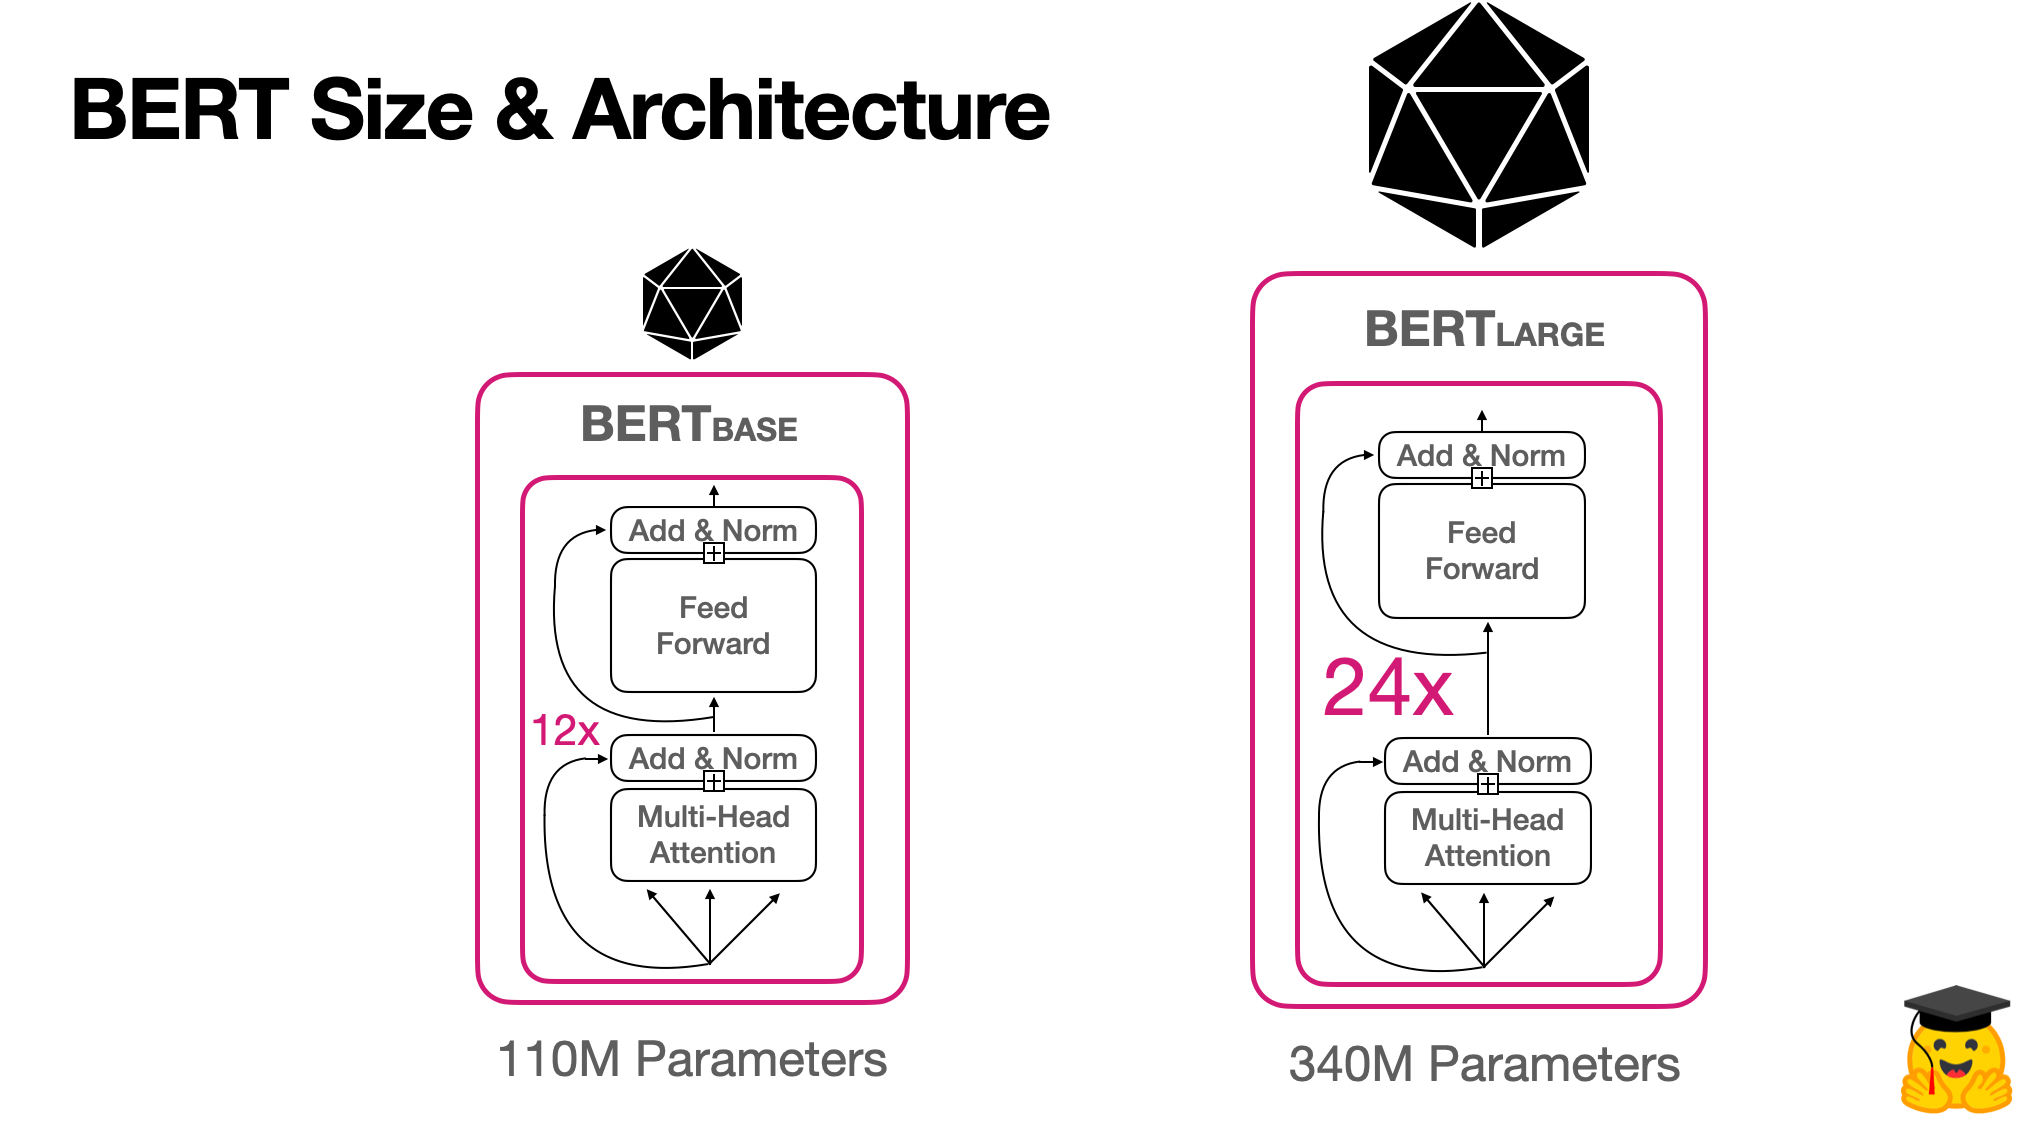
\includegraphics[width=0.8\textwidth]{images/bert.png}
    \caption{Архитектура BERT}
    \label{fig:bert_architecture}
\end{figure}

В рекомендательных системах BERT и его варианты используются главным образом для кодирования контента и учёта последовательности действий. Например, модель BERT4Rec \citep{sun2019bert4rec} адаптировала архитектуру BERT для последовательных рекомендаций: например, история просмотров пользователя можно рассматривать как последовательность «слов», и BERT-энкодер обучался предсказывать пропущенные элементы этой последовательности \footnote{Foundation Model for Personalized Recommendation // URL: \url{https://netflixtechblog.com/foundation-model-for-personalized-recommendation-1a0bd8e02d39}}. Такая модель успешно улавливает сложные паттерны в последовательностях взаимодействий, превзойдя классические методы на откртых датасетах рекомендаций. Кроме того, BERT применяется для извлечения признаков из пользовательских отзывов и описаний товаров – интеграция этих семантических признаков доказала свою пользу в улучшении качества рейтинговых прогнозов


\textbf{GPT (Generative Pre-trained Transformer)} - семейство авторегрессивных моделей-декодеров, генерирующих текст последовательностью слева направо. В отличие от BERT, GPT-модели обучаются предсказывать следующий токен на основе предыдущих, что делает их исключительно мощными в генерации последовательностей и продолжений контекста \citep{zhao2024recommendersystemsin}. Обучение GPT-моделей обычно основано на максимизации правдоподобия следующего токена по всему обучающему корпусу. Функция потерь для авторегрессионного языкового моделирования может быть выражена следующим образом:
\[ \mathcal{L}_{LM}(\theta) = - \sum_{t=1}^{|S|} \log P(w_t | w_1, w_2, \dots, w_{t-1}; \theta) \]
где \(S = (w_1, w_2, \dots, w_{|S|})\) – это последовательность токенов, а \(\theta\) – параметры модели. Модель предсказывает каждый токен \(w_t\), основываясь на предыдущих токенах \((w_1, \dots, w_{t-1})\).
В задачах рекомендации он применяется разными способами. С одной стороны, GPT можно обучить генерировать список рекомендуемых объектов по описанию предпочтений пользователя. Такой подход используется в интерактивных сценариях: например, LLM может по запросу в свободной форме (natural language prompt) последовательно сгенерировать названия треков или фильмов, подходящих под запрос, как будто продолжая диалог с пользователем \citep{palumbo2025text2trackspromptbasedmusicrecommendation}. Однако прямая генерация названий объектов сопряжено с трудностями: модель может ошибаться в названиях, требуется дополнительный шаг сопоставления текста с конкретными ID контента, а длина генерируемых имен замедляет вывод списка. Поэтому в промышленных реализациях генеративный подход видоизменяется – например, модель Text2Tracks (Spotify) предлагает генерировать сразу идентификаторы треков в нужном формате в обход прямой генерации названий. С другой стороны, GPT нашёл применение для диалоговых рекомендательных систем и генерации объяснений. Появление крупной модели ChatGPT показало, что языковой интеллект может вести сложные диалоги, включая сценарий «рекомендательного чат-бота». Исследователи активно эксперементируют с большими языковыми моделями в данной форме, что привело к созданию таких моделей как Chat-REC \citep{gao2023chatrec}, использующую ChatGpt как основу рекомендационного движка. В целом, GPT-архитектуры открыли возможность генеративных рекомендательных систем, где модель буквально пишет рекомендации как ответ на запрос, обогащая опыт пользователя (например, может предложить подборку товаров в форме связного описательного ответа, а не просто списка). 

\textbf{T5 (Text-To-Text Transfer Transformer)} - архитектура энкодер-декодер, разработанная командой Google, в которой любая задача обработки текста представляется в формате «текст на входе – текст на выходе». T5 обучается унифицированно решать разные NLP-задачи, превращая, например, классификацию в задачу порождения слова "positive" или "negative" в ответ на промпт с отзывом, и т.д. Модель обучается с использованием стандартной функции потерь для последовательностей (sequence-to-sequence), такой как перекрестная энтропия, по всему набору разнообразных текстовых задач. Обучающая цель T5 может быть представлена как:
\[ \mathcal{L}_{Seq2Seq}(\theta) = - \sum_{(X, Y) \in \mathcal{D}} \sum_{t=1}^{|Y|} \log p_\theta(y_t | y_{<t}, X) \]
где \(X\) – входная текстовая последовательность (например, задача с инструкцией), \(Y = (y_1, \dots, y_{|Y|})\) – целевая текстовая последовательность, \(\mathcal{D}\) – обучающий набор данных, а \(\theta\) – параметры модели. Модель генерирует каждый токен целевой последовательности \(y_t\), основываясь на предыдущих токенах этой последовательности \(y_{<t}\) и полной входной последовательности \(X\). Такая универсальность оказалась востребованной и в рекомендациях: на базе T5 была создана серия моделей, позволяющих единым образом решать множество рекомендательных задач. Пример – модель P5 (Personalized Prompted PLM), где предобученный T5 взят за основу и дообучен на различных задачах рекомендаций одновременно \citep{geng2022recommendationaslanguageprocessing}. Для этого все данные (матрица взаимодействий, профили пользователей, тексты обзоров, описания товаров) были сконвертированы в текстовые шаблоны-подсказки (prompts). Пользователи и объекты в этих промптах представлены специальными токенами-идентификаторами (например, \texttt{<user\_123>} для пользователя, \texttt{<item\_1>} для объекта), которые добавляются в словарь модели как новые уникальные слова. Модель P5 затем обрабатывает эти текстовые последовательности для генерации требуемого ответа. Например, процесс рекомендации следующего товара для пользователя \texttt{<user\_123>} после взаимодействий с \texttt{<item\_1>} и \texttt{<item\_2>} можно представить так:
\begin{itemize}
    \item \textbf{Входной промпт (Input Prompt):} Текстовая последовательность, кодирующая запрос пользователя и его историю.
    \begin{center}
    \texttt{<user\_123> liked <item\_1>, <item\_2>. Recommends: ?}
    \end{center}
    \item \textbf{Выход модели (Model Output):} Сгенерированный моделью специальный токен, представляющий идентификатор рекомендуемого товара.
    \begin{center}
    \texttt{<item\_42>}
    \end{center}
\end{itemize}
Здесь \texttt{<item\_42>} — это сгенерированный моделью идентификатор рекомендуемого товара. Благодаря этой схеме один и тот же T5 научается выполнять сразу несколько функций: топ-N рекомендацию, предсказание рейтингов, генерацию текстовых рекомендаций и даже объяснений, просто получая разный текстовый промпт на входе. Подход P5 продемонстрировал, что универсальная LLM может заменить множество узкоспециализированных моделей рекомендаций, если грамотно сформулировать их ввод/вывод в виде текста. Помимо P5, появляются и другие крупные модели, адаптированные под рекомендации: например, M6-Rec – мультимодальный трансформер с сотнями миллиардов параметров, применённый для персонализации в e-commerce (Alibaba) \citep{cui2022m6recgenerativepretrainedlanguage}. В целом, архитектуры типа T5 особенно полезны там, где требуется совместить несколько источников данных (текст, рейтинги, профили) и выйти за рамки простого ранжирования – то есть позволяют обобщить разные задачи рекомендации в едином текстовом пространстве.

Помимо вышеперечисленных, в исследовательских работах фигурируют и другие архитектуры и семейства моделей. Например, XLNet (успешно применялся для понимания отзывов), Albert и DistilBERT (облегчённые версии BERT), а в новейших работах используются даже диалоговые модели вроде GPT-4/ Gemini Pro. Однако базовые принципы остаются схожими: рекомендации получают выгоду либо от энкодеров, способных тонко анализировать содержание (BERT, RoBERTa и пр.), либо от генеративных декодеров, способных выдавать последовательности в виде рекомендаций или пояснений (GPT-семейство, LLaMA и др.), либо от их комбинации (T5, FLAN-T5, etc.), объединяющей понимание и генерацию.


\subsection*{Фреймворки и платформы для интеграции LLM в рекомендательные системы}
\addcontentsline{toc}{subsection}{Фреймворки и платформы для интеграции LLM в рекомендательные системы}

Активное развитие методов на стыке NLP и рекомендательных систем привело к появлению специализированных библиотек, облегчающих использование LLM в рекомендациях.

Базовой платформой является библиотека Hugging Face Transformers, предоставляющая предобученные модели (GPT, BERT, T5) и средства для их тонкой настройки на данных рекомендаций. Однако для специфических задач рекомендательных систем требуются дополнительные компоненты.

Специализированным решением стал пакет NVIDIA Merlin Transformers 4Rec для последовательных и сессионных рекомендаций. Библиотека интегрируется с экосистемой HuggingFace и предоставляет готовые модули: позиционные эмбеддинги, механизмы маскирования последовательностей, оптимизированное многоголовое внимание. На её основе созданы улучшенные версии BERT4Rec и SASRec, показавшие state-of-the-art результаты.

Для промышленного применения развиваются облачные платформы. Amazon Bedrock включает модель Titan Embeddings, преобразующую текстовые описания товаров в эмбеддинги для использования в рекомендательных движках реального времени. Это позволяет заменить сложные конвейеры обработки текста единым вызовом LLM-модели.

В исследовательской сфере доступны фреймворки Microsoft Recommenders с реализацией BERT4Rec, библиотека RecBole и LangChain для построения диалоговых рекомендателей через цепочки вызовов LLM. 

\subsection*{Актуальные исследования}
\addcontentsline{toc}{subsection}{Актуальные исследования}
Развитие в области больших языковых моделей неприменно приводит к появлению новых исследований, связанных с их применением в рекомендательных системах. 
Например, исследование "Reason4Rec: Крупные языковые модели для рекомендаций с совещательным согласованием предпочтений пользователя" фокусируется на устранении недостатков поверхностного анализа, характерных для современных рекомендательных систем, построенных на основе больших языковых моделей (RecLLM).
Авторы отмечают, что такие системы часто напрямую предсказывают отклик пользователя, не углубляясь в явный процесс рассуждения о его предпочтениях. Этот подход "быстрого мышления" может приводить к ошибкам в сложных ситуациях, чувствительности к смещениям в данных и трудностям с обобщением \citep{fang2025reason4rec}

В качестве решения предлагается концепция "Совещательной Рекомендации" (Deliberative Recommendation). Суть ее в том, чтобы обучить LLM проходить через явный этап обдумывания и генерации рассуждений о предпочтениях пользователя и характеристиках товара перед тем, как сделать окончательное предсказание. Важным элементом этого подхода является использование 'вербализованной обратной связи пользователя', такой как текстовые отзывы, в качестве обучающих сигналов для формирования процесса рассуждения LLM. Этот фреймворк декомпозирует сложный процесс рассуждения на три последовательных этапа, каждый из которых выполняется специализированным экспертным модулем. Эти эксперты реализованы как отдельные адаптеры QLoRA на одной и той же базовой LLM, что позволяет снизить вычислительные затраты

\begin{figure}[H]
    \centering
    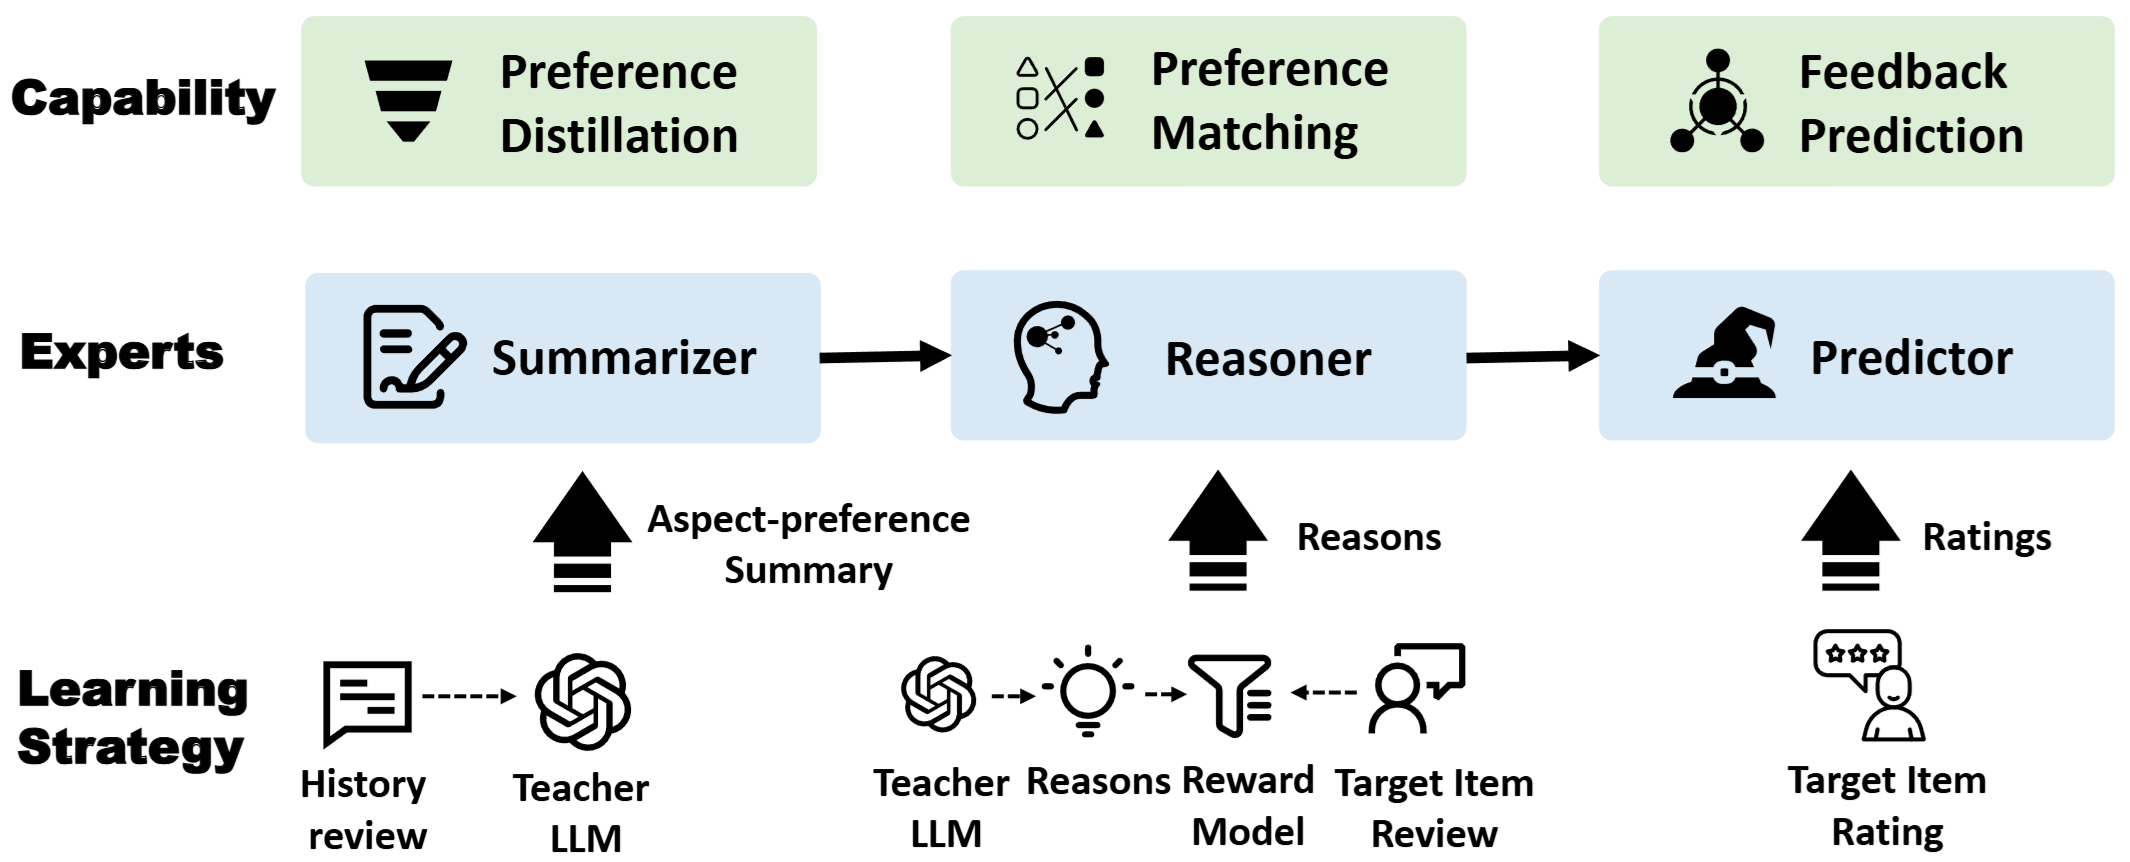
\includegraphics[width=0.8\textwidth]{reason_4_rec.png}
    \caption{Архитектура модели Reason4Rec}
    \label{fig:reason4rec}
\end{figure}

Иной подход к решению проблемы поверхностного анализа можно обнаружить в статье LLMs for User Interest Exploration in Large-scale Recommendation Systems \citep{wang2024llms}. Традиционные рекомендательные системы часто попадают в "ловушку обратной связи". Они учатся на том, что вы делали в прошлом, и рекомендуют похожее. Это мешает открывать для себя что-то совершенно новое и может привести к "усталости от контента".

Данная статья предлагает использовать большие языковые модели (LLM) для того, чтобы помочь пользователям исследовать новые области интересов, выходящие за рамки их привычных предпочтений. Идея в том, чтобы LLM, обладающая обширными знаниями о мире, подсказывала, какие новые направления могут быть интересны пользователю, а уже классическая рекомендательная система подбирала бы конкретные элементы (например, видео, товары) в рамках этих новых направлений.

Авторами предлагается гибридная двухуровневая система:

Верхний уровень (LLM – Стратег):
\begin{itemize}
    \item Вместо того чтобы LLM пыталась предсказать конкретный следующий товар (что сложно и дорого для огромных каталогов), она работает с более крупными "кластерами интересов". Эти кластеры – это группы товаров, объединенных общей темой (например, "Кластер 1: Автобусы, Грузовики, Дороги...", "Кластер 2: Кокос, Банан, Фрукты...").
    \item LLM получает на вход информацию о недавних кластерах интересов пользователя (например, "Недавно я смотрел видео из Кластера 1 и Кластера 2").
    \item Ее задача – сгенерировать описание нового кластера интересов, который мог бы понравиться пользователю, но который отличается от его недавней истории. Например, LLM может предложить: "Новый кластер: Акулы, Подводный мир, Дайвинг...".
    \item Важно, что LLM специально дообучается (fine-tuning) так, чтобы ее текстовые описания новых интересов точно соответствовали одному из заранее определенных кластеров в системе ("контролируемая генерация").
\end{itemize}

Нижний уровень (Классическая рекомендательная система – Тактик):
\begin{itemize}
    \item Получив от LLM описание нового кластера интересов (и его ID), классическая система (например, трансформерная модель последовательных рекомендаций) подбирает уже конкретные товары/видео.
    \item Ключевой момент: поиск товаров ограничивается только теми, которые входят в предложенный LLM новый кластер. Это обеспечивает персонализацию в рамках нового направления.
\end{itemize}

Взяв за основу данное исследование, мы попытались реализовать его на основе данных из открытых источников, а также open-source LLM.  % Обзор литературы
\newpage

\section*{Построение модели}
\addcontentsline{toc}{section}{Построение модели}

\subsection*{Описание используемых данных}
\addcontentsline{toc}{subsection}{Описание используемых данных}

В нашем исследовании мы использовали открытый набор данных MTS Kion Implicit Contextualised Sequential Dataset for Movie Recommendation. Он включает 5 476 251 запись о взаимодействиях 962 179 пользователей с 15 706 фильмами. Для каждого сеанса просмотра в нём указаны метка времени, продолжительность и процент досмотра. Кроме того, датасет содержит демографические сведения о пользователях (пол, возраст, уровень дохода, наличие детей) и подробные метаданные о фильмах — жанры, ключевые слова, актерский состав, режиссеры и другие характеристики.

Датасет состоит из трех основных файлов:
\begin{itemize}
    \item \texttt{Interactions.csv} - фиксирует неявные взаимодействия пользователей с контентом, включая долю и время просмотра.
    \item \texttt{Users.csv} - включает демографические характеристики пользователей (пол, возрастная категория, доходы, наличие детей).
    \item \texttt{Items.csv} - содержит метаданные контента (название, оригинальное название, год производства, жанры, ключевые слова, описания, страны и студии производства, актерский состав, режиссеры).
\end{itemize}

Ключевые статистики датасета:
\begin{itemize}
    \item Количество пользователей: 962,179
    \item Количество объектов (фильмов): 15,706
    \item Количество взаимодействий: 5,476,251
    \item Среднее количество взаимодействий на одного пользователя: 5.69
    \item Разреженность данных: 99.9\%
\end{itemize}

\subsection*{Предобработка данных}
\addcontentsline{toc}{subsection}{Предобработка данных}
В ходе работы была выполнена предварительная обработка трех основных наборов данных (users, items, interactions) и данных для сабмита с использованием библиотеки polars. Ключевые этапы включали:
\begin{itemize}
    \item \textbf{Анализ и обработка пропущенных значений}: 
    Для каждого датафрейма были выявлены и обработаны пропуски. В категориальных признаках (например, возраст, пол, доход пользователей; оригинальное название, страны, студии у объектов) пропуски заменялись специальными метками (например, "age non specified", "Unknown") или наиболее подходящими значениями на основе анализа данных (например, 0 для watched pct или for kids).
    \item \textbf{Преобразование типов данных}:
    Многие колонки были преобразованы в более эффективные или семантически корректные типы. Категориальные строковые признаки (возраст, пол, доход, тип контента, жанры и др.) были переведены в тип Enum для оптимизации памяти и производительности. Числовые флаги (например, kids flg) преобразованы в булев тип. Даты (last watch dt) были переведены в формат Datetime.
    \item \textbf{Стандартизация текстовых данных}:
    Текстовые поля, такие как названия фильмов (title, title orig), стран, студий, режиссеров и актеров, были приведены к нижнему регистру и очищены от лишних пробелов. Для полей с множественными значениями (например, 'countries', 'studios') была применена стандартизация путем разделения, уникализации, сортировки и объединения значений.
    \item \textbf{Инженерия признаков}:
    На основе года выпуска фильмов (release year) был создан новый категориальный признак release year range, группирующий фильмы по десятилетиям.
    \item  \textbf{Проверка целостности}:
    После всех преобразований была выполнена проверка на отсутствие пропущенных значений в обработанных датафреймах.
    \item  \textbf{Сохранение результатов}:
    Очищенные и предобработанные датафреймы (users, items, interactions) были сохранены в эффективном формате Parquet для дальнейшего использования в исследовании.

    В целом, предобработка была направлена на улучшение качества данных, их консистентности и пригодности для последующего анализа и моделирования.
\end{itemize}

\subsection*{Создание текстовых эмбеддингов}
\addcontentsline{toc}{subsection}{Создание текстовых эмбеддингов}

Последующей задачей после предобработки данных является создание текстовых эмбеддингов каждого фильма. Для этого мы первым делом должны создать уникальное текстовое описание для каждого фильма. Для этого мы используем следующие поля:
\begin{itemize}
    \item \textbf{title}: Название фильма
    \item \textbf{genres}: Жанры фильма
    \item \textbf{kw}: Ключевые слова фильма
    \item \textbf{plot}: Описание фильма
    \item \textbf{countries}: Страны производства
    \item \textbf{studios}: Студии, производящие фильм
    \item \textbf{actors}: Актеры, сыгравшие в фильме
    \item \textbf{age rating}: Возрастной рейтинг фильма
\end{itemize}

Примером такого описания может служить следующий текст:
\begin{minted}[fontsize=\small,frame=single,label=Пример текстового описания фильма]{text}
title: поговори с ней
genres: драмы, зарубежные, детективы, мелодрамы
kw: трагедия, любовь, комедия, легендарный, педро
plot: мелодрама легендарного педро альмодовара
directors: педро альмодовар
actors: адольфо фернандес, ана фернандес, 
release_year: 2000-2010
age_rating: 16.0
\end{minted}

Первоначальный анализ существующих ключевых слов в датафрейме items df показал их неоптимальность для задачи создания эмбеддингов из-за дублирования информации из других полей (например, страна выпуска) и не всегда корректного разделения фраз.

Для решения этой проблемы было принято решение сгенерировать новые, более релевантные ключевые слова с помощью большой языковой модели (LLM). В качестве LLM была выбрана модель google/gemma-3-4b-it. Для генерации ключевых слов был разработан специальный промпт, состоящий из системного сообщения (SYSTEM MSG), инструктирующего модель выступать в роли эксперта-аналитика фильмов, и пользовательского промпта (build user prompt), который передавал модели название фильма (оригинальное и локализованное), жанры и описание. Инструкции для модели включали:

\begin{itemize}
    \item Сгенерировать до 8-10 ключевых слов или коротких фраз.
    \item Сфокусироваться на темах, сеттинге и атмосфере контента.
    \item Избегать общих слов (фильм, сериал, год, актеры).
    \item Выводить результат в виде списка, разделенного запятыми.
\end{itemize}

Генерация производилась батчами по 64 объекта для эффективности. Для каждого объекта формировался полный промпт, токенизировался, и модель model.generate создавала новые ключевые слова с параметрами max new tokens=50, do sample=True, temperature=0.3. Сгенерированные ключевые слова (generated\_keywords) были добавлены в исходный датафрейм items df в колонке kw.

На основе логики создания эмбеддингов, описанной раннее, а также сгенерированных ключевых слов было создано единое текстовое описание для каждого объекта, предназначенное для последующего получения векторных представлений (эмбеддингов).

Для преобразования текстовых описаний embedding\_text в векторные представления использовалась модель SentenceTransformer 'jina embeddings v3'. Это многоязычная многозадачная модель текстовых эмбеддингов, предназначенная для широкого спектра задач обработки естественного языка. Модель основана на архитектуре Jina-XLM-RoBERTa. Эмбеддинги генерировались батчами по 256 текстов, с последующей нормализацией и преобразованием в numpy массивы типа float32. Из полных эмбеддингов были отобраны первые 256 компонент для каждого объекта (emb\_256) для последующей кластеризации.

Качество полученных 256-мерных эмбеддингов оценивалось на основе их способности группировать семантически схожие объекты, используя жанровую информацию в качестве прокси-меры.
Была рассчитана матрица косинусного сходства (sim) между всеми парами эмбеддингов объектов. Для каждого объекта было найдено K=10 ближайших соседей.

Метрики оценки включали:
\begin{itemize}
    \item \textbf{Genre Hit-Rate@10}: Доля объектов, у которых хотя бы один из 10 ближайших соседей разделяет общий жанр. Полученное значение составило 0.987.
    \item \textbf{Mean Intra-Genre Similarity}: Среднее косинусное сходство между парами объектов, принадлежащих одному и тому же жанру. Это значение (0.400) сравнивалось со средним сходством между случайными парами объектов из разных кластеров (Mean inter sim = 0.282), что подтвердило хорошую семантическую группировку эмбеддингов. Дополнительно была проведена выборочная ручная проверка нескольких кластеров (на данном этапе еще не формализованных, а основанных на ближайших соседях) путем анализа их текстовых описаний.
\end{itemize}

\subsection*{Иерархическая кластеризация}
\addcontentsline{toc}{subsection}{Иерархическая кластеризация}

Для дальнейшего анализа и кластеризации объектов был использован алгоритм иерархической кластеризации. В качестве меры близости использовалось расстояние между эмбеддингами
\begin{itemize}
    \item \textbf{Построение k-NN графа}: Эмбеддинги объектов были L2-нормализованы. С использованием библиотеки faiss был создан индекс IndexFlatIP для эффективного поиска ближайших соседей по скалярному произведению (эквивалентно косинусному сходству для нормализованных векторов). Для каждого объекта было найдено K=50 ближайших соседей. На основе этой информации был сформирован датафрейм edges, представляющий собой k-NN граф с указанием источника (src), цели (dst) и косинусного сходства (cosine).

    \item \textbf{Учет "трафика" объектов}: Из датафрейма взаимодействий (interactions) для каждого item\_id был рассчитан 'трафик' как сумма общей длительности просмотров (total\_dur). Эти данные были сохранены в словаре traffic\_map.

    \item \textbf{Алгоритм balanced-split}: Был реализован рекурсивный алгоритм иерархической кластеризации. Целевое количество кластеров L2 было установлено в 320 (TARGET L2), максимальная глубина дерева – 9 (MAX DEPTH), максимальное и минимальное количество объектов в листовом кластере – 120 (MAX ITEMS) и 6 (MIN ITEMS) соответственно. Алгоритм итеративно разделял группы объектов на два подкластера с помощью KMeans (примененного к эмбеддингам), пока не достигались критерии остановки: максимальная глубина, целевой суммарный трафик листа или минимальное количество объектов в листе.

    \begin{algorithm}
    \caption{Алгоритм balanced-split кластеризации}
    \label{alg:balanced_split}
    \small
    \begin{algorithmic}[1]
    \Procedure{BalancedSplit}{$ids$, $traffic$, $vecs$, $L2$, $D$, $MAX$, $MIN$}
    \State $trf \gets \sum_{i \in ids} traffic.get(i)$; $max\_trf \gets trf / L2$
    \State $id2idx \gets \{id: idx \text{ for } (idx, id) \text{ in } enumerate(ids)\}$
    \State $clusters \gets \emptyset$; $stack \gets [(ids, 0)]$
    \While{$stack$ не пуст}
        \State $(nodes, depth) \gets stack.pop()$
        \State $leaf\_trf \gets \sum_{n \in nodes} traffic.get(n)$
        \If{$(depth = D)$ \textbf{or} $(leaf\_trf \leq max\_trf \text{ and } |nodes| \leq MAX)$ \textbf{or} $(|nodes| \leq MIN)$}
            \State добавить $nodes$ в $clusters$; \textbf{continue}
        \EndIf
        \State $X \gets vecs[[id2idx[n] \text{ for } n \in nodes]]$
        \State $labels \gets \Call{KMeans}{X, k=2}$
        \State $left, right \gets$ разделить $nodes$ по $labels$
        \If{$left$ пуст \textbf{or} $right$ пуст}
            \State добавить $nodes$ в $clusters$
        \Else
            \State $stack.append((left, depth + 1)); stack.append((right, depth + 1))$
        \EndIf
    \EndWhile
    \State \textbf{return} $clusters$
    \EndProcedure
    \end{algorithmic}
    \end{algorithm}
\end{itemize}

В результате было сформировано 249 кластеров L2 (листовых кластеров).
Пример одного из полученных кластеров:

\begin{quote}
\textbf{Кластер 124} | размер=99
\begin{itemize}
    \item \textit{пламя - я твоя тень} — жанры: драмы; ключевые слова: первобытный мир, огонь, борьба за выживание, примитивная пара, драка, выжив...
    \item \textit{таинственный сад} — жанры: семейное, фэнтези, приключения; ключевые слова: таинственный сад, магическое место, детство, приключе...
    \item \textit{ковчег} — жанры: приключения, детективы, драмы, зарубежные, фантастика; ключевые слова: фантастический сериал, ковчег, полярная...
    \item \textit{наваждение} — жанры: драмы, триллеры, детективы; ключевые слова: потеря, горе, спасение заложников, двойник, подозрение, италия...
\end{itemize}
\end{quote}

Что касается основных метрик кластеризации, то они получились следующими:
\begin{itemize}
    \item Коэффициент вариации "трафика" по кластерам составил 0.56, указывая на приемлемую сбалансированность.
    \item Среднее внутрикластерное косинусное сходство (0.453) оказалось заметно выше межкластерного (0.282), что свидетельствует о хорошем качестве разделения.
    \item Также был проведен ручной анализ содержимого нескольких случайных кластеров.
\end{itemize}

\subsection*{Извлечение ключевых слов кластеров}
\addcontentsline{toc}{subsection}{Извлечение ключевых слов кластеров}
Для каждого из 249 полученных L2 кластеров были извлечены характеризующие их ключевые слова.

\begin{itemize}
    \item Загружен датафрейм с результатами предыдущего этапа.
    \item В качестве текстовой основы для каждого объекта использовалась колонка core\_text (алиас для generated\_keywords, полученных от LLM).
    \item Тексты core\_text всех объектов внутри одного кластера были объединены в единый документ для этого кластера.
    \item Для каждого такого документа кластера с помощью TfidfVectorizer (с токенизацией nltk.word\_tokenize для русского языка, n-граммами (1, 2), min\_df=2, max\_features=50000) были рассчитаны TF-IDF веса слов и фраз.
    \item Для каждого кластера L2 были отобраны топ-5 ключевых слов/фраз с наибольшими TF-IDF значениями.
\end{itemize}

\subsection*{Подготовка данных для моделирования переходов между кластерами}
\addcontentsline{toc}{subsection}{Подготовка данных для моделирования переходов между кластерами}

На основе полученных кластеров и данных о взаимодействиях пользователей был сформирован датасет для задачи предсказания следующего кластера, который может заинтересовать пользователя.

\begin{itemize}
    \item Загружены данные о взаимодействиях пользователей и ключевых словах кластеров.
    \item Взаимодействия были отфильтрованы по проценту просмотра (watched pct >= 70).
    \item Для каждого пользователя была построена временная последовательность уникальных кластеров L2, с которыми он взаимодействовал.
    \item На основе этих последовательностей были созданы примеры для обучения: "промпт", содержащий ключевые слова двух предыдущих кластеров в последовательности, и "таргет" – ключевые слова следующего кластера в последовательности.
    \item Полученный датасет был сбалансирован путем ограничения количества примеров (до 10) для каждого уникального таргет-кластера, чтобы уменьшить влияние наиболее популярных кластеров. Изначальный размер 1,188,204 записей был сокращен до 2,449.
\end{itemize}

Пример полученного промпта для модели:

\begin{figure}[h]
\centering
\begin{tcolorbox}[
    colback=gray!5,
    colframe=gray!50,
    boxrule=1pt,
    arc=2pt,
    left=10pt,
    right=10pt,
    top=10pt,
    bottom=10pt,
    width=0.9\textwidth
]
\small\ttfamily
The films or series I watched most recently are in the following clusters:

\textbf{Cluster 1:} каледония, новая каледония, океан, биоразнообразие, гондурас

\textbf{Cluster 2:} индонезия, гондурас, природа, папуа, леса

Each cluster is described with salient phrases or entity names.
With less than 30 words, generate a new and different cluster I will watch next
with highly specific salient phrases or entity names, with a prefix that says "New cluster: "

\textbf{New cluster:} южная африка, африка, южная, дикая, дикая природа
\end{tcolorbox}
\caption{Пример промпта для модели предсказания следующего кластера.}
\label{fig:prompt_example}
\end{figure}

\section*{Моделирование переходов между кластерами}
\addcontentsline{toc}{section}{Моделирование переходов между кластерами}
Далее рассмотрим процесс дообучения большой языковой модели на сформированных промптах переходов между кластерами контента. Основная цель данного этапа заключается в адаптации предобученной модели к специфике задачи предсказания пользовательских предпочтений в области видеоконтента.

Для решения поставленной задачи был выбран подход fine-tuning существующей языковой модели, что позволяет использовать накопленные знания о языке и семантических связях, одновременно специализируя модель под конкретную предметную область. В качестве базовой архитектуры была выбрана модель "meta-llama/Llama-3.1-8B-Instruct", которая представляет собой инструкционно-настроенную версию модели Llama 3.1 с 8 миллиардами параметров.

Выбор данной модели обусловлен несколькими факторами:

\begin{itemize}
    \item Высокая эффективность в задачах следования инструкциям и генерации структурированного текста.
    \item Размер модели в 8 миллиардов параметров обеспечивает оптимальный баланс между качеством генерации и вычислительными требованиями.
    \item Открытая лицензия позволяет проводить дообучение и модификацию модели для исследовательских целей.
\end{itemize}

Процесс дообучения осуществляется на подготовленном датасете промптов переходов, где каждый пример содержит описание двух предыдущих кластеров в истории просмотров пользователя и целевой кластер, который пользователь выбрал следующим. Такая структура данных позволяет модели изучить паттерны пользовательского поведения и семантические связи между различными типами контента. Примеры сформированных промптов представлены на рисунке \ref{fig:prompt_example}.

\subsection*{Архитектура LoRA для эффективного дообучения}
\addcontentsline{toc}{subsection}{Архитектура LoRA для эффективного дообучения}

Для дообучения языковой модели Llama-3.1-8B-Instruct была применена архитектура LoRA (Low-Rank Adaptation), которая представляет собой эффективный метод параметрически-эффективного обучения больших языковых моделей.

LoRA основана на гипотезе о том, что изменения весов предобученной модели во время дообучения имеют низкий внутренний ранг. Вместо обновления всех параметров модели, LoRA добавляет обучаемые матрицы низкого ранга к существующим весам линейных слоев.

Для линейного слоя с весовой матрицей $W_0$, LoRA представляет обновление весов как:

\begin{equation}
W = W_0 + \Delta W = W_0 + BA
\end{equation}

где $B$ и $A$ — обучаемые матрицы низкого ранга $r$.

Основные преимущества LoRA:
\begin{itemize}
    \item Значительное сокращение количества обучаемых параметров
    \item Отсутствие дополнительной задержки во время инференса
    \item Возможность быстрого переключения между различными адаптерами
\end{itemize}

В нашем эксперименте использовались следующие параметры:
\begin{itemize}
    \item Ранг адаптации: $r = 16$
    \item Масштабирующий фактор: $\alpha = 32$
    \item Целевые модули: слои внимания и выходные проекции
\end{itemize}

Применение LoRA позволило сократить количество обучаемых параметров с 8,198,033,408 до 167,772,160 (2.05\% от общего количества), при этом сохранив высокое качество дообучения для задачи предсказания пользовательских предпочтений
Для обучения такого количества параметров была использована GPU Nvidia A100 40GB.

\subsection*{Параметры дообучения}
\addcontentsline{toc}{subsection}{Параметры дообучения}

Для дообучения модели были использованы следующие ключевые параметры:

\begin{itemize}
    \item \textbf{Размер батча}: 20 примеров на устройство с накоплением градиента через 2 шага (эффективный batch size = 40)
    \item \textbf{Количество эпох}: 10
    \item \textbf{Скорость обучения}: $2 \times 10^{-4}$ с разогревом в течение 10\% шагов
    \item \textbf{Оптимизатор}: AdamW
    \item \textbf{Точность вычислений}: bfloat16 для экономии памяти
    \item \textbf{Максимальная длина последовательности}: 512 токенов
    \item \textbf{Метрика для выбора лучшей модели}: article\_match\_rate
\end{itemize}

\subsection*{Метрики оценки модели}
\addcontentsline{toc}{subsection}{Метрики оценки модели}

Для оценки производительности дообученной языковой модели в задаче генерации рекомендаций следующего кластера интересов пользователя были использованы следующие метрики:

\textbf{1. recall\_exact\_completion (Точность полного совпадения)}

Данная метрика измеряет долю случаев, в которых текстовое описание кластера, сгенерированное моделью, полностью и дословно совпадает с эталонным описанием следующего кластера из тестового набора данных.

\begin{equation}
\text{recall\_exact\_completion} = \frac{N_{\text{полных совпадений}}}{N_{\text{всего примеров}}}
\end{equation}

где $N_{\text{полных совпадений}}$ — количество примеров, для которых предсказание модели идентично эталону, а $N_{\text{всего примеров}}$ — общее количество примеров в тестовом наборе. Метрика отражает способность модели к точному воспроизведению целевых последовательностей.

\textbf{2. avg\_jaccard\_to\_true (Средняя схожесть по ключевым словам с эталоном)}

Эта метрика оценивает среднюю степень семантического пересечения между набором ключевых слов, извлеченных из сгенерированного моделью описания кластера, и набором ключевых слов из эталонного описания кластера.

Для каждого примера извлекаются множества ключевых слов из предсказания модели ($K_{pred}$) и из эталона ($K_{true}$). Вычисляется индекс Жаккара:

\begin{equation}
J(K_{pred}, K_{true}) = \frac{|K_{pred} \cap K_{true}|}{|K_{pred} \cup K_{true}|}
\end{equation}

Итоговая метрика является средним значением индекса Жаккара по всем примерам тестового набора:

\begin{equation}
\text{avg\_jaccard\_to\_true} = \frac{1}{N_{\text{всего примеров}}} \sum_{i=1}^{N_{\text{всего примеров}}} J(K_{pred, i}, K_{true, i})
\end{equation}

Метрика характеризует, насколько предложенные моделью ключевые слова релевантны ожидаемым.

\textbf{3. article\_match\_rate (Соответствие критериям статьи)}

Ключевая метрика, оценивающая соответствие предсказания модели двум основным критериям: предложенный кластер должен быть (а) семантически отличным от двух предыдущих кластеров, показанных пользователю, и (б) семантически схожим с одним из существующих в системе валидных кластеров.

Для каждого примера:
\begin{itemize}
    \item Извлекается набор ключевых слов из предсказания модели ($K_{pred}$)
    \item Из промпта извлекаются наборы ключевых слов для двух предыдущих кластеров ($K_{prev1}$, $K_{prev2}$)
    \item Проверяется условие отличия: 
    \begin{align}
    J(K_{pred}, K_{prev1}) &< \text{порог}_{\text{отличия}} \text{ И} \\
    J(K_{pred}, K_{prev2}) &< \text{порог}_{\text{отличия}}
    \end{align}
    (например, $\text{порог}_{\text{отличия}} = 0.8$)
    \item Проверяется условие валидности: существует хотя бы один кластер $K_{valid}$ из общего списка валидных кластеров системы, для которого $J(K_{pred}, K_{valid}) \geq \text{порог}_{\text{валидности}}$ (например, $\text{порог}_{\text{валидности}} = 0.8$)
\end{itemize}

Если оба условия (отличие и валидность) выполнены, предсказание засчитывается как "match". Итоговая метрика:

\begin{equation}
\text{article\_match\_rate} = \frac{N_{\text{article matches}}}{N_{\text{всего примеров}}}
\end{equation}

Эта метрика отражает способность модели предлагать пользователю новые и одновременно релевантные интересы, соответствующие известным категориям.

\subsection*{Результаты дообучения}
\addcontentsline{toc}{subsection}{Результаты дообучения}

В процессе дообучения модели, как уже было отмечено, отслеживались ключевые метрики качества на валидационном наборе данных. Получившиеся результаты обучения представлены в таблице \ref{tab:training_results}.

\begin{table}[H]
\centering
\caption{Результаты дообучения модели по шагам}
\label{tab:training_results}
\small
\begin{tabular}{|c|c|c|c|c|}
\hline
\textbf{Шаг} & \textbf{Train Loss} & \textbf{Match Rate} & \textbf{Recall} & \textbf{Jaccard} \\
\hline
100 & 0.0779 & 0.9531 & 0.1694 & 0.2407 \\
\hline
200 & 0.0568 & 0.9918 & 0.3510 & 0.4058 \\
\hline
300 & 0.0496 & 0.9959 & 0.3857 & 0.4326 \\
\hline
400 & 0.0471 & 0.9939 & 0.3918 & 0.4394 \\
\hline
\end{tabular}
\end{table}

Анализ результатов показывает следующее:

\begin{itemize}
    \item \textbf{Снижение training loss}: Наблюдается устойчивое снижение потерь на обучающем наборе с 0.0779 до 0.0471, что свидетельствует об эффективном обучении модели.
    
    \item \textbf{Стабильность validation loss}: Потери на валидационном наборе остаются относительно стабильными (около 0.45), что указывает на отсутствие переобучения.
    
    \item \textbf{Высокие значения Article Match Rate}: Ключевая метрика достигает хороших результатов — от 95.3\% на 100-м шаге до 99.6\% на 300-м шаге, демонстрируя способность модели генерировать семантически корректные и отличающиеся от предыдущих кластеры.
    
    \item \textbf{Улучшение точности воспроизведения}: Метрика Recall Exact Completion показывает рост с 16.9\% до 39.2\%, отражая повышение способности модели к точному воспроизведению целевых описаний.
    
    \item \textbf{Рост семантической схожести}: Средний индекс Жаккара увеличивается с 0.24 до 0.44, что указывает на улучшение качества генерируемых ключевых слов.
\end{itemize}

\textbf{Пример работы модели}

Для демонстрации качества генерируемых рекомендаций приведем пример взаимодействия с дообученной моделью:

\begin{figure}[H]
\centering
\begin{tcolorbox}[
    colback=gray!5,
    colframe=gray!50,
    boxrule=1pt,
    arc=2pt,
    left=10pt,
    right=10pt,
    top=10pt,
    bottom=10pt,
    width=0.9\textwidth
]
\small\ttfamily
\textbf{Prompt:} The films or series I watched most recently are in the following clusters:

\textbf{Cluster 1:} война, отечественная война, отечественная, великая отечественная, летчики

\textbf{Cluster 2:} месть, драма, боевик, бои, спорт

Each cluster is described with salient phrases or entity names.
With less than 30 words, generate a new and different cluster I will watch next
with highly specific salient phrases or entity names, with a prefix that says "New cluster: "

\textbf{Предсказание:} New cluster: расследование, разруха, убийство, смоленск, советский детектив
\end{tcolorbox}
\caption{Пример работы дообученной модели.}
\label{fig:model_example}
\end{figure}

Данный пример демонстрирует способность модели генерировать семантически связанные, но отличающиеся от исходных кластеры, учитывая предпочтения пользователя к военной тематике и драматическим произведениям.

\subsection*{Создание lookup-таблицы для инференса}
\addcontentsline{toc}{subsection}{Создание lookup-таблицы для инференса}

После успешного дообучения модели следующим шагом стало создание эффективного механизма для практического применения модели в условиях реального времени. Для этого была разработана lookup-таблица, содержащая предвычисленные предсказания для всех возможных пар предыдущих кластеров.

\textbf{Процесс создания lookup-таблицы}

Идея заключается в том, чтобы для каждой возможной комбинации двух предыдущих кластеров предсказать следующий кластер с помощью дообученной LLM и сохранить эти соответствия. Процесс включает следующие этапы:

\begin{itemize}
    \item \textbf{Генерация всех возможных пар}: Из полученных 249 кластеров L2 формируются все возможные комбинации пар $(cluster_i, cluster_j)$, где $i, j \in \{1, 2, ..., 249\}$.
    
    \item \textbf{Создание промптов}: Для каждой пары кластеров автоматически генерируется промпт в том же формате, который использовался при обучении модели.
    
    \item \textbf{Генерация предсказаний}: Дообученная модель обрабатывает каждый промпт и генерирует предсказание следующего кластера.
    
    \item \textbf{Сохранение соответствий}: Результаты сохраняются в виде таблицы соответствий вида $(cluster_{prev1}, cluster_{prev2}) \rightarrow cluster_{next}$.
\end{itemize}

\textbf{Архитектура предлагаемого пайплайна}

На основе созданной lookup-таблицы может быть разработан эффективный пайплайн рекомендательной системы:

\begin{figure}[H]
\centering
\begin{tikzpicture}[node distance=1.5cm]
    % Определение стилей
    \tikzset{
        start/.style={rectangle, rounded corners, minimum width=2cm, minimum height=1cm, text centered, draw=black, fill=blue!20},
        process/.style={rectangle, minimum width=2.5cm, minimum height=1cm, text centered, draw=black, fill=orange!20},
        decision/.style={rectangle, minimum width=2cm, minimum height=1cm, text centered, draw=black, fill=green!20},
        endpoint/.style={rectangle, rounded corners, minimum width=2.5cm, minimum height=1cm, text centered, draw=black, fill=red!20},
        arrow/.style={thick,->,>=stealth}
    }

    % Узлы
    \node (user) [start] {User ID};
    \node (history) [decision, below of=user] {30-day history};
    \node (lookup) [process, below of=history] {Lookup table};
    \node (cluster) [process, below of=lookup] {Next cluster};
    \node (mask) [decision, below of=cluster] {SASRec / Bert4Rec};
    \node (items) [endpoint, below of=mask] {Top-N items};

    % Стрелки
    \draw [arrow] (user) -- (history);
    \draw [arrow] (history) -- node[anchor=west] {last 2 clusters} (lookup);
    \draw [arrow] (lookup) -- (cluster);
    \draw [arrow] (cluster) -- (mask);
    \draw [arrow] (mask) -- (items);
\end{tikzpicture}
\caption{Схема предлагаемого пайплайна рекомендательной системы}
\label{fig:pipeline}
\end{figure}

Предлагаемый пайплайн должен работать следующим образом:

\begin{enumerate}
    \item \textbf{Извлечение истории пользователя}: По User ID получается 30-дневная история взаимодействий пользователя.
    
    \item \textbf{Определение последних кластеров}: Из истории выделяются уникальные последние 2 кластера, с которыми взаимодействовал пользователь.
    
    \item \textbf{Поиск в lookup-таблице}: По паре предыдущих кластеров в предвычисленной таблице находится рекомендуемый следующий кластер.
    
    \item \textbf{Применение SASRec}: Используется предобученная модель SASRec с маскированием логитов для генерации рекомендаций только из объектов целевого кластера.
    
    \item \textbf{Формирование рекомендаций}: Возвращается список Top-N наиболее релевантных объектов из предсказанного кластера.
\end{enumerate}

\textbf{Преимущества данного подхода}

Использование lookup-таблицы обеспечивает:

\begin{itemize}
    \item \textbf{Высокую скорость инференса}: Устраняется необходимость в реальном времени запускать тяжелую LLM для генерации предсказаний.
    
    \item \textbf{Предсказуемую латентность}: Время отклика системы становится константным и не зависит от сложности модели.
    
    \item \textbf{Масштабируемость}: Система может обслуживать большое количество пользователей одновременно без дополнительных вычислительных затрат на LLM.
    
    \item \textbf{Простоту развертывания}: Не требуется специализированная инфраструктура для запуска больших языковых моделей в продакшене.
\end{itemize}

Полученные результаты подтверждают эффективность применения LoRA-архитектуры для дообучения большой языковой модели в задаче генерации персонализированных рекомендаций контента, а также решению проблемы замкнутости рекомендательной системы.

\textbf{Направления дальнейших исследований}

Следующим этапом исследования было бы проведение онлайн-эксперимента для сравнения производительности дообученной языковой модели с классическими подходами к рекомендациям. В качестве базовых методов для сравнения целесообразно рассмотреть:

\begin{itemize}
    \item \textbf{Hierarchical Contextual Bandit} — метод, использующий иерархическую структуру для моделирования контекстных предпочтений пользователей
    \item \textbf{Collaborative Filtering} — классические алгоритмы коллаборативной фильтрации
    \item \textbf{Content-based методы} — рекомендации на основе содержательных характеристик объектов
    \item \textbf{Гибридные подходы} — комбинирующие различные методы рекомендаций
\end{itemize}

Онлайн-тестирование позволило бы оценить реальное влияние предлагаемого подхода на пользовательский опыт, измерить метрики вовлеченности (время просмотра, количество кликов, конверсия) и проверить способность модели решать проблему замкнутости рекомендательных систем в реальных условиях эксплуатации.
 % Модель
\newpage
\section*{Заключение}
\addcontentsline{toc}{section}{Заключение}

В рамках данного исследования была разработана и экспериментально апробирована методология применения больших языковых моделей для решения задачи персонализированных рекомендаций контента. Проведенная работа включала несколько ключевых этапов: от предобработки данных и создания семантических представлений до дообучения языковой модели и оценки её эффективности.

Основные результаты исследования:

\begin{itemize}
    \item \textbf{Успешная реализация гибридного подхода}: Разработанная двухуровневая архитектура, объединяющая иерархическую кластеризацию контента на основе текстовых эмбеддингов и дообученную языковую модель для генерации переходов между кластерами, продемонстрировала высокую эффективность.
    
    \item \textbf{Высокие показатели качества}: Дообученная модель Llama-3.1-8B с архитектурой LoRA достигла значения Article Match Rate на уровне 99.6\%, что свидетельствует о способности генерировать семантически корректные и отличающиеся от предыдущих рекомендации.
    
    \item \textbf{Эффективность параметрически-экономичного обучения}: Применение LoRA позволило сократить количество обучаемых параметров до 2.05\% от общего объема модели при сохранении высокого качества дообучения.
    
    \item \textbf{Решение проблемы замкнутости}: Предложенный подход успешно адресует классическую проблему замкнутости рекомендательных систем, позволяя пользователям исследовать новые области интересов за пределами их привычных предпочтений.
    
    \item \textbf{Масштабируемость решения}: Использование кластеризации контента и работа на уровне семантических групп, а не отдельных объектов, обеспечивает возможность применения подхода к каталогам различного размера.
\end{itemize}

Проведенный анализ показал, что интеграция больших языковых моделей в рекомендательные системы открывает новые возможности для создания более интеллектуальных и адаптивных решений. LLM продемонстрировали способность к пониманию сложных семантических связей между различными типами контента и генерации релевантных рекомендаций на основе ограниченного контекста.

Развитие больших языковых моделей в задачах рекомендаций выглядит крайне многообещающим. Возможности современных LLM в области понимания естественного языка, способности к обобщению и контекстному рассуждению создают предпосылки для революционных изменений в области персонализации контента. Ожидается, что дальнейшее совершенствование архитектур языковых моделей, методов их обучения и интеграции с традиционными рекомендательными подходами приведет к созданию нового поколения рекомендательных систем, способных обеспечить более глубокое понимание пользовательских потребностей и предоставить качественно новый уровень персонализированного опыта.

Результаты данной работы вносят вклад в понимание практических аспектов применения LLM в индустриальных рекомендательных системах и могут служить основой для дальнейших исследований в этой динамично развивающейся области.


\newpage



\bibliographystyle{plainnat}
\bibliography{bibliography}

\end{document}